\documentclass[12pt]{report}

% Paquetes necesarios
\usepackage[utf8]{inputenc} % Codificación UTF-8
\usepackage[spanish]{babel} % Idioma español
\usepackage{graphicx}       % Para incluir imágenes
\usepackage{hyperref}       % Hipervínculos
\usepackage{geometry}       % Configurar márgenes
\usepackage{titlesec}       % Modificar títulos
\usepackage{fancyhdr}       % Encabezados y pies de página
\usepackage{gensymb}
\usepackage{textcomp}
\usepackage{upquote}
\usepackage{svg}
%\setlength{\parindent}{1.5em}
% Configuración de márgenes
\geometry{a4paper, margin=1in}
\graphicspath{{img/}}
\addto\captionsspanish{\renewcommand{\tablename}{Tabla}}
\addto\captionsspanish{\renewcommand{\listtablename}{Índice de Tablas}}

% Configuración de hipervínculos

\hypersetup{
    colorlinks=true,
    linkcolor=blue,
    urlcolor=blue,
    citecolor=blue,
    pdftitle={Título de la Tesis},
    pdfauthor={Tu Nombre}
}

% Configuración del encabezado y pie de página
%\pagestyle{fancy}
%\fancyhf{}
%\fancyhead[L]{Título de la Tesis}
%\fancyhead[R]{\thepage}
%\fancyfoot[C]{Nombre del Autor}

% Configuración de los títulos
\titleformat{\chapter}[hang]{\bfseries\Large}{\thechapter.}{1em}{}

% Inicio del documento

% Inicio del documento
\begin{document}

% Portada
\begin{titlepage}
    \centering
    {\Huge {Universidad de la Habana}}\\[1cm]
    {\Huge {Facultad de Matemática y Computación }}\\[0.5cm]
 
    \begin{figure}[h]
    	\centering
    	
\includegraphics[width=0.3\textwidth]{logoUH.png}
    \end{figure}
    {\noindent\hrulefill}\\[0.2cm]
    
    {\Large\textbf{{Test para detectar patrones DIAG y LINE  en las contraseñas gráficas de PassPoint, basado en el promedio de los ángulos máximos de los triángulos de Delaunay, condicionado al número de triángulos }}}\\[0.1cm]
    {\noindent\hrulefill}\\[1.0cm]
    \begin{minipage}{0.8\textwidth}
    \begin{center}
    	{\Large Trabajo de Diploma presentado en opción al título de Licenciado en Ciencias de la Computación}
    	
    \end{center}
    \end{minipage}\\[1cm]
    
    
 
    
    {\Large {Autor: Ovidio Navarro Pazos}}\\[2cm]
   	{\Large {Tutores: M.Sc. Lisset Suárez Plasencia}}\\
   	\hspace{7.5em}{\Large{Dr.C. Carlos Miguel Legón Pérez}}\\
   	\hspace{7.5em}{\Large{M.Sc. Joaquín A. Herrera Macías}}\\
   	[2.0cm]
   	
   	{\large{La Habana, Cuba}}\\
    {\large  \today}
\end{titlepage}




\chapter*{Resumen}
\hypertarget{Resumen}{}

	Un método de autenticación que difiere de las contraseñas alfanuméricas tradicionales es la autenticación gráfica. Una de las técnicas más valiosas dentro de este campo es PassPoint, conocida por su equilibrio entre seguridad y usabilidad. Sin embargo, esta técnica puede ser vulnerada si el usuario sigue patrones predefinidos al seleccionar los cinco puntos en la imagen, como los patrones DIAG y LINE. Investigaciones previas han destacado la utilidad de las características de las triangulaciones de Delaunay para extraer información de estos puntos que constituyen la contraseña, siendo el AMADT (promedio de los ángulos máximos de los triángulos de Delaunay) una de estas características relevantes.
	
	En este estudio, se comparan contraseñas gráficas generadas por la elección aleatoria de cinco puntos en una imagen con contraseñas que siguen patrones específicos del tipo DIAG y LINE. La comparativa se basa en segmentar las contraseñas que siguen estos patrones, considerando el número de triángulos en sus triangulaciones de Delaunay (3, 4 o 5). Experimentalmente se demuestra que, para cada número de triángulos, las contraseñas con patrones DIAG y LINE tienen un AMADT más alto que aquellas generadas con puntos aleatorios. Estudios previos respaldan este resultado y sugieren la viabilidad de un test de aleatoriedad espacial para identificar contraseñas gráficas débiles que sigan los patrones DIAG y LINE, utilizando el AMADT como estadístico. Se estiman las distribuciones más adecuadas para cada número de triángulos y se lleva a cabo el test para evaluar los errores de tipo I y tipo II.
	La relevancia de este test radica en la similitud de los resultados con pruebas previas. Sería crucial determinar si estos hallazgos son redundantes o complementarios para mejorar la seguridad del sistema de autenticación gráfica PassPoint.


\chapter*{Abstract}
\hypertarget{Abstract}{}
	One authentication method that differs from traditional alphanumeric passwords is graphical authentication. One of the most valuable techniques within this field is PassPoint, known for its balance between security and usability. However, this technique can be breached if the user follows predefined patterns when selecting the five dots in the image, such as the DIAG and LINE patterns. Previous research has highlighted the usefulness of Delaunay triangulation features to extract information from these points that constitute the password, with AMADT (average of the maximum angles of the Delaunay triangles) being one of these relevant features.
	
	In this study, graphical passwords generated by randomly choosing five points in an image are compared with passwords that follow specific patterns of the DIAG and LINE type. The comparison is based on segmenting the passwords that follow these patterns, considering the number of triangles in their Delaunay triangulations (3, 4 or 5). Experimentally it is shown that, for each number of triangles, passwords with DIAG and LINE patterns have a higher AMADT than those generated with random dots. Previous studies support this result and suggest the feasibility of a spatial randomization test to identify weak graphical passwords following DIAG and LINE patterns, using AMADT as a statistic. The best-fitting distributions for each number of triangles are estimated and the test is carried out to assess type I and type II errors.
	The relevance of this test lies in the similarity of the results with previous tests. It would be crucial to determine whether these findings are redundant or complementary to improve the security of the PassPoint graphical authentication system.

% Índice
\tableofcontents
\newpage
\listoffigures
\newpage
\listoftables


% Capítulos
\chapter*{Introducción}
\addcontentsline{toc}{chapter}{Introducción}
\hypertarget{introduccion}{}


	En la actualidad, la gran mayoría de los usuarios tienden a ignorar las recomendaciones de seguridad al momento de crear sus contraseñas. Es común observar el uso por los usuarios de contraseñas cortas y cargadas de información personal, lo cual facilita su memorización, pero aumenta significativamente su vulnerabilidad frente a ataques de fuerza bruta o de diccionario \cite{1,2,3,4}.
	
	Debido a esta inherente contradición entre facilidad y seguridad que presentan las contraseñas alfanuméricas, se han desarrollado nuevos métodos alternativos de autenticación, entre los que se encuentran los métodos basados  en contraseñas gráficas. Este nuevo enfoque surge por la capacidad humana de recordar patrones visuales en una imagen con mayor facilidad que largas cadenas de caracteres alfanuméricos aleatorios. En este tipo de contraseñas, el usuario debe recordar una imagen o partes específicas de ella mediante la selección  de determinados puntos.
	% No obstante, no cualquier imagen  puede ser seleccionada para emplearse en este metodo, se deben escoger imágenes que posean cientos de Hotspots[6](puntos probales de ser seleccionados) dispersos en la misma. Lo que equivale a decir que posea un amplio tamaño de espacio de contraselas, y de este modo ser más resistentes a los ataques comunes.
	%tratar de agregar hospoto puntos probabless
	%$imágenes que dadas sus características posean un amplio espacio para la construcción de sus contraseñas y de este modo ser más resistentes a los ataques de diccionarios, obteniendo un espacio de búsqueda mucho más amplio y resistente a los ataques comunes.
	
	El sistema PassPoint\cite{1} es un método de autenticación gráfica que destaca por su usabilidad y seguridad. Este método consiste  en que el usuario seleccione en la fase de registro  cinco puntos de una imagen elegida por el usuario o dada por el sistema. Durante la autenticación, el usuario debe hacer click en una determinada vecindad y en el mismo orden de los puntos seleccionados en la fase de  registro. Una de las debilidades de este sitema es que los usuarios tienden a seleccionar los Hotspots\cite{4}(puntos más probables a seleccionar en una imagen), por esta razón las imágenes usadas en el sistema tienen que poseer cientos de Hotspots dispersos de manera homegénea. Además existen un conjunto de patrones no aleatorios que tienden a seguir los usuarios y su combinación con los Hotspots sería un grave error pues hace que la contraseña sea muy susceptible a ataques de diccionarios. Estos patrones incluyen formas específicas como Z, W, C, V, patrones agrupados, regulares y los que más suelen seleccionar los usuarios  que son los  patrones DIAG o LINE\cite{5}(formas de diagonales o línea)
	
	%Entre las debilidades de esta técnica se encuentran los Hotspots[6](puntos más probables a seleccionar por el usuario), además diversos patrones predefinidos que los usuarios tienden a seguir durante el registro para facilitar la memorización. Estos patrones incluyen formas específicas como Z, W, C, V, patrones agrupados o regulares, y patrones LOD, DIAG o LINE (formas de línea o diagonales).
	
	La tendencia de los usuarios a crear patrones entre los puntos seleccionados, ya sea de manera independiente o en combinación con Hotspots, constituye una debilidad importante. Por ello, resulta fundamental desarrollar tests que detecten la existencia de estos patrones en las contraseñas antes de su uso, ya que contribuirían significativamente a mejorar la seguridad de la técnica PassPoint.
	
	

	A lo largo de los últimos años, se han realizado pocas investigaciones enfocadas en este tema. Entre los métodos más comunes para evaluar la Aleatoriedad Espacial Completa se encuentran: el test de la función K-Ripley, el test de la función G, que analiza la distancia al vecino más cercano, y el test de la función F, que se centra en la distancia de espacio vacío. Sin embargo, en \cite{6,7} se demuestra que, en el contexto de PassPoint, dos de estos métodos son ineficaces para detectar contraseñas gráficas compuestas por patrones agrupados. Por otro lado, en \cite{7,8} se evidencia que los tres tests no logran identificar ni el agrupamiento ni la regularidad en las contraseñas de este escenario. Hasta ahora, en la bibliografía revisada, se han encontrado 4 tests efectivos \cite{7,9,10,11} para identificar contraseñas no aleatorias que presentan patrones agrupados o regulares en el contexto de PassPoint. Estos métodos se basan, en el caso de \cite{9}, en el promedio de los perímetros de los triángulos de Delaunay, en  \cite{7} en la distancia media entre cinco puntos, para el caso de \cite{10} es una aplicación conjunta de los tests \cite{7,9}, y \cite{11} basado en  el perímetro de la envoltura convexa. De estos tests \cite{11} es el más efectivo encontrado en la literatura y el segundo más eficiente después de \cite{7}.
	
	Teniendo en consideración \cite{12}, las propiedades de una triangulación de Delaunay brindan la capacidad de obtener información acerca de la interrelación entre puntos, se ha empleado como una herramienta en la mitad de la década de 1980 para identificar configuraciones de puntos. En el estudio realizado por Chiu en \cite{12}, se emplearon varias de estas propiedades para reconocer la agrupación y la regularidad entre los puntos. Específicamente, la característica del ``ángulo máximo de un triángulo de Delaunay", según la literatura revisada, nunca había sido utilizada previamente para identificar otro tipo de configuraciones además de las agrupadas o regulares. No obstante, dado que los patrones DIAG y LINE se distinguen por presentar un ángulo cercano a 0{\degree } entre dos segmentos consecutivos o en otras palabras que las curvas formadas entre los 5 puntos sean curvas suaves a pedazos, es decir, que carezca de picos.  De ahí que, en \cite{13} se propuso y demostró que la media de los ángulos máximos de los triángulos de Delaunay generados a partir de los puntos de las contraseñas gráficas de PassPoint es un estadígrafo eficaz para detectar la presencia de patrones DAIG y LINE, incluso con un número limitado de puntos. En \cite{5} se entendía como el ángulo formado entre dos segmentos consecutivos, el menor de los dos ángulos que forman la intersección de la prolongación de los segmentos de una contraseña. En este trabajo se referirá al mayor de estos dos ángulos como el ángulo adyacente entre dos segmentos .


	
	Según los resultados obtenidos en \cite{13}, la distribución del promedio de los triángulos de  Delaunay de las contraseñas gráficas aleatorias, sin tener en cuenta el número específico de triángulos sigue una distribución Normal, por lo que se plantea la hipótesis de que cada una de las distribuciones de los conjuntos cuyas triangulaciones contienen 3, 4 o 5 triángulos también distribuirán Normal pero con diferentes parámetros. Suponiendo que esta hipótesis se cumpla, dada una contraseña ingresada por un usuario se verificará a que distibución pertenece y se aplicará el test con la distribución adecuada. Esto debería mejorar el ajuste de los datos a los test de bondad de ajuste y aumentar la efectividad del test.
	% se sugiere investigar la eficacia de un test de detección de los patrones DIAG y LINE  utilizando como estadígrafo el promedio de los ángulos máximos de los triángulos de Delaunay, pero realizando análisis independientes según el número de triángulos en su triangulación (3,4 o 5) y realizar un análisis comparativo respecto a los resultados obtenidos en \cite{13}.\\
	
	\large{\textbf{Problema de investigación:}}
	
	\normalsize{¿Cómo  detectar contraseñas gráficas que sigan patrones DIAG y LINE  en el sistema de autenticación gráfica PassPoint, teniendo en cuenta el número de triángulos de Delaunay?}\\
	
	\large{\textbf{Objeto de estudio:}}
	
	\normalsize{Número de triángulos de las  triangulaciones de Delaunay  en autentificación gráfica}\\
	
		   
	\large{\textbf{Campo de acción:}}
	
	\normalsize{Detección de contraseñas gráficas que sigan patones DIAG y LINE en el escenario PassPoint   utilizando  el número de triángulos de las triagulaciones de Delaunay}.\\
	 
	\large{\textbf{Hipótesis:}}

	\normalsize{Es posible detectar contraseñas gráficas que sigan patrones DIAG y LINE en el sistema de autenticación gráfica Passpoint, teniendo en cuenta el número de triángulos  de las triangulaciones de Delaunay}.\\
		
	
	\large{\textbf{Idea de la solución:}}
	
	\normalsize{
		%Para cada cantidad de triángulos  en las triangulaciones de Delaunay para 5 puntos:
		Debido a que en la bibliografía existe un test capaz de detectar patrones DIAG y LINE en las contraseñas gráficas de PassPoint basado en el promedio de los ángulos máximos de los triángulos de Delaunay. Se propone construir un test para detectar este tipo de patrones en las contraseñas gráficas en dicho escenario, pero teniendo en cuenta el número de triángulos de la triangulación de Delaunay correspondiente. Con el fin de llegar a comparar ambos test en cuanto a efectividad, y realizar la aplicación conjunta de ambos si es posible para lograr una mayor efectividad en la detección de estos tipos de patrones.
		}\\

	\large{\textbf{Objetivos:}}
	
	\normalsize{\textbf{Objetivos generales}}: Detectar las contraseñas gráficas que siguen patrones DIAG o LINE en PassPoint para cada número de triángulos en una triangulación de Delaunay.
	
	\normalsize{\textbf{Objetivos específicos}}:
	Para cada número de triángulos  en las triangulaciones de Delaunay de 5 puntos:
	
	\begin{itemize}
		\item Encontrar cómo distribuye el promedio de los ángulos máximos de la triangulación de Delaunay en contraseñas aleatorias.
		\item Construir un test de aleatoriedad basado en la distribución del promedio de los ángulos máximos de los triángulos de Delaunay en contraseñas aleatorias.
		
		\item Realizar un análisis estadístico con las estimaciones de los errores tipo I y tipo II cometidos para validar.
		
		\item Realizar una comparación con los resultados obtenidos en \cite{13}.
		
	\end{itemize}
	
	
	{\large{\textbf{Estructura de la tesis}}}\\
	
	Este trabajo estará dividido en dos capítulos.
	
	En el primero se muestra la en que consiste la técnica de autenticación gráfica PassPoint, así como sus ventajas y desventajas, se describen los patrones comunes que los usuarios suelen seguir al crear sus contraseñas, destacando los patrones DIAG y LINE, se definen las triangulaciones de Delaunay y sus propiedades. Por último se raliza un resumen de \cite{13}, el cual demuestra que el promedio de los ángulos máximos de los  triángulos de Delaunay es un estadígrafo eficaz para detectar patrones DIAG y LINE en contraseñas de PassPoint.
	
	En el segundo capítulo se investiga el promedio de los ángulos máximos de los triángulos de Delaunay en función del número de triángulos que conforman dicha triangulación. Tomando en cuenta el tamaño estándar de las imágenes(1920x1080) para cada posible número de triángulos presentes en las triangulaciones de Delaunay de las contraseñas de 5 puntos(3,4 o 5) se estiman las  mejores distribuciones a las que se ajustan y se propone un test de detección de patrones DIAG y LINE en PassPoint para estimar los errores de tipo I y tipo II. Posteriormente, se realiza una comparación de los resultados obtenidos y los hallazgos presentados en el estudio\cite{13}.
	
	
	
	
	

%%buscar en tesis de lisset los tipos de ataques
\setcounter{chapter}{0}
\chapter{Marco Teórico}
Incluye el marco teórico, revisiones de la literatura y conceptos clave relacionados con tu trabajo.
En esta sección se definen los conceptos clave que son relevantes para este trabajo. 

\section{PassPoint}
	La técnica PassPoint diseñada por Wiedenbeck(77 osviel) destaca entre los sistemas de autenticación gráfica del tipo cued-recall por su usabilidad y seguridad(rodrigez et al..2018 comparacion pag3) .
	%usabilidad
	Esta técnica consiste en que  en su fase de registro el
	usuario debe seleccionar 5 puntos(pixeles) de una imagen ya sea seleccionada por el mismo usuario o dada por el sistema  y en el proceso de autenticación este debe hacer click en el mismo orden y en determinada  vecindad o región de tolerancia de los puntos escogidos en la fase de registro.
	%parte de hotspot
	Wiedenbeck su investigación (77 osviel) asegura que las imágenes más deseadas para el proceso debían tener contenido que tuviera significado para el usuario por lo que debían tener escenas concretas, otro requisito es que la imagen seleccionada posean cientos de HOTSPOST(puntos más probables a seleccionar por el usuario o mejor llamados puntos calientes) diseminados de forma homogénea, pero existe el problema de que en el momento de autentificación el usuario no seleccione exactamente el mismo punto y a esto se le llaman errores de discretización, esta se encarga de establecer una tolerancia alrededor de cada punto, por tanto esto disminuye el espacio de contraseñas y aumenta información relevante a la hora de los ataques de diccionarios. Se puede encontrar un análisis sobre la relevancia del mecanismo de discretización en los sistemas de contraseñas gráficas en [75, 76, 77 Liset]. Por otro lado, en [75, 76, 77, 78 Liset] se describen los distintos métodos de discretización que se han desarrollado hasta ahora.\\
	\begin{figure}[ht]
		\centering
		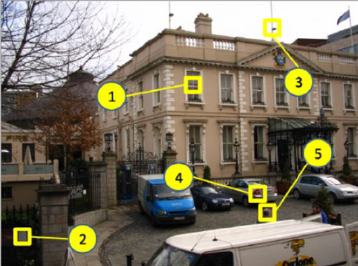
\includegraphics[width=0.5\textwidth]{passpoint.png}
		\caption{PassPoint.}
		\label{fig:PassPoint}
	\end{figure}
	
	%Una discusion acerca de la importancia del mecanismo de discretizacion en los esquemas de contrsaseñas graficas puede verse en [75,76,77 lisset], mientras que en [75,76,77,78 liset] pueden verse los diferentes metodos de discretizacion conocidos hasta el momento sad
	
	%modelo para hotspot
	En el trabajo (3 sensor) se presenta un método que permite determinar si una imagen es adecuada para ser utilizada en esta técnica. Este método conduce al desarrollo de un modelo diseñado para identificar las regiones de una imagen que los usuarios tienen mayor probabilidad de elegir como parte de sus contraseñas. Según sus experimentos, el modelo puede predecir puntos de interés (Hotspots) con una precisión de entre el 70 \% y el 80 \%, aunque el tamaño de la muestra utilizada es limitado. La aplicación de esta técnica en el sistema PassPoint sería especialmente útil para mejorar la confiabilidad en la asignación de imágenes. Por otro lado, en el estudio (4 sensor) se demostró que incluso un pequeño cambio en la imagen puede influir en la elección de contraseñas por parte del usuario durante la fase de registro, afectando así su nivel de seguridad.    

	%espacio de contrase;as osviel
	%En cuanto al espacio, segun (77 osviel) no se necesitarian muchos puntos para hacer la contraseña segura, con 5 o 6(en una imagen de 1024x725) se puede lograr mas que contraseñas que con 8 caracteres dentro del un alfebeto estandar de 64 letras. En la tabla (graphical vs alphanumeric) tomada de una investigacion se puede apreciar una comparacion entre los espacios de contraseñas graficas y alfanumericas variando el alfabeto , la longitud de la contraseña,tolerancia y tamaño de la imagen. Se puede apreciar que para 5 puntos y un tamaño de imgen razonable las contraseñas gráficas conservan un espacio de clave superior a las alfanumericas
	
	En relación al espacio de contraseñas, según (77 Osviel), no sería necesario utilizar muchos puntos para crear una contraseña segura. Con solo 5 o 6 puntos (en una imagen de 1024x725), se podría lograr mayor seguridad que con contraseñas de 8 caracteres dentro de un alfabeto estándar de 64 símbolos. En la tabla (Graphical vs Alphanumeric), se muestra una comparación entre los espacios de contraseñas gráficas y alfanuméricas, considerando factores como el alfabeto, la longitud de la contraseña, la tolerancia y el tamaño de la imagen. Se observa que, con 5 puntos y un tamaño de imagen razonable, las contraseñas gráficas mantienen un espacio de clave superior al de las contraseñas alfanuméricas.
	
\begin{table}[h!]
	\centering
	\begin{tabular}{|c|c|c|c|c|c|}
		\hline
				 	 
		         		 & Image size &   Grid square &	Alphabet size/ &Lenght/No.  & Password \\ 
		                &           &  size(pixels)  & No.squares& click points & space size \\ \hline
		Alphanumeric    & N/A       & N/A     & 64   & 8  & 2.8x \\ \hline
		Alphanumeric    & N/A       & N/A     & 72   & 8  & 7.2x10 \\ \hline
		Alphanumeric    & N/A       & N/A     & 96   & 8  & 7.2x10 \\ \hline
		Graphical        & 451x331   & 20x20   & 373  & 5  &7.2x10 \\ \hline
		Graphical        & 1024x752  & 20x20   & 1925 & 5  &2.6x10 \\ \hline
		Graphical        & 1024x752  & 14x14   & 3928 & 5  &9.3x10 \\ \hline
		Graphical(1/2   & 1024x752  & 14x14   & 1964 & 5  & 2.9x10 \\ 
		screen used)   &   &    &  &  &  \\ \hline
	\end{tabular}
	\caption{Alfanuméricas vs Gráficas}
	\label{tabla:Alfanuméricas vs Gráficashhh}
\end{table}


	%tolerancia(discretizacion)
	

	
	
	
	%vantajas y desventajas
	
	%Gran n´umero de usuarios en las contrase˜nas gr´aficas tienden a seleccionar contrase˜nas que siguen determinados patrones, esto ayuda a la memorabilidad de las contrase˜nas pero al mismo tiempo contribuye a que sea relativamente f´acil encontrar un diccionario de ataque a este tipo de patrones. Como siguen cierto patr´on se les denomina contrase˜nas d´ebiles porque carecen de aleatoriedad. Ahora veremos cuales son los distintos patrones que tienden a seleccionar los usuarios a la hora de confeccionar sus contrase˜nas[3]

\section{Patrones en contraseñas gráficas}
Además de la inclusión por parte de los usuarios de los Hotspots en las contraseñas, estas presentan otro tipo de debilidades como son los distintos tipos de patrones, leyes psicológicas o modelos de atención visual, los cuales son comunmente utlizados por los usuarios para garantizar una mejor memorabilidad, lo que hace que sea más fácil contruir diccionarios de ataques estas contraseñas.
Algunos de los patrones reportados en la literatura[15-21 sensor] son: los patrones con una forma predeterminada(Z, W, V, C), los agrupados,  los regulares,y los patrones LOD y DIAG(o patrones diagonales) en los que se encuentran los patrones LINE(forma de línea). 
Los patrones DIAG y LINE(fig de diag y line) se encuentran entre los que más tienden a seguir los suarios, en[16-21 sensors] caracterizan los patrones DIAG  por ser puntos que se encuentran formando arcos tanto horizontal como verticalmente y la suma de los valores absolutos de los ángulos es menor que 15\degree[7 informe de sensor], en cambio los LINE se caracterizan por ser lineas horizontales y verticales y se definen como un subconjunto de los DIAG. 
\textbf{FIGURA DE DIAG Y LINE}.
\\
En[17,18 sensor] tras realizar un estudio de 223 contraseñas graficas en el escenario PassPoint seleccionadas por estudiantess en dos imagenes diferentes con un numero asequible de Hotspots distribuidos uniformemente en cada una de ellas, los autores consiguieron obtener del 48.2\% al 54.1\% de las mismas utilzando un ataque de diccionario de 235.26 entradas utilizando patrones  DIAG y del 23.7\% al 52.3\% de dichas contraseñas utilizando un ataque de 229.02 entradas utilizando  patrones LINE 


%que me diga esto con otras palabras 
%toda la biblio de estas subsecciones son de  2018 scnc
%\subsection{Modelos de atención}
%Los Modelos Visuales De Atencion(MVA) estudian la forma en que las personas observan una imagen. Se estima que un grupo significativo de usuariios escoge los puntos siguiendo estos patrones (14). De esta manera se pueden construir dicccionarios con los grupos de puntos mas probables a seleccionar por el usuario.
%Los modelos computacionales de atencion Botton-Up, se definen normalmente por caracteristicas de las imagenes digitales tales como: la intensidad, el color y la orientacion(9,12). Por otra partelos modelos computacionales TopDown, pueden ser definidos por entrenamiento. La dificultad de estos ultimos se basa en que la tarea Top-down debe ser predefinida(ej.encontrar personas en una imagen) en um grupo de imagenes que se etiquetan con areas que contienen a los sujetos (14). Nos enfocaremos en la la propuesta de Itti(8,9) ya que exsite evidencia empírica  de que este captura la forma en que las persinas observan una imagen desde lo profundo hacia arriba(botton-up)(13). La idea principal de esta propuesta es que algunas areas de una imagen, son salientes o de alguna manera resaltan por que difieren del resto de su entorno. De esta manera dada una imagen  ek modelo devuelve las localizzaciones y el orden en que el ser humano de forma insconciente y automatica la observa. El proceso se compone de dos etapas. En la primera se crea un mapa de salientes basados en las caracteristicas visuales. En la segunda etapa se usa una red neuronal 'winner-take-wall' con el objetivo de replicar la forma en que el usuario observaria la imagen. En(15) se desarrolla un ataque automatico de diccionario que se basaba solo en variaciones de la primera etapa donde utilizaba deteccion de esquinas para encontrar puntos referenciables, luego en (14) se describe como seria la segunda etapa del proceso.
%La idea principal ( primera etapa ) de esto metodo sirve de soporte para las tecnocas de analisis y procesamiento de imagenes. Estas se vasen en la deteccion de esquinas y centroides asi como la plicacion de herramientas y algoritmos de inteligencia artificial para detectar objetos en imagenes

\section{Triangulaciones de Delaunay}
\textbf{Definición(Triángulación de Delaunay):}Una triangulación del conjunto P de los puntos sobre el plano es de Delaunay, si y sólo si la circunferencia circunscrita de cualquier triángulo en la red no contiene un punto p en su interior,como muestra la figura(triangulacionnes ). Esta condición es conocida como condición de Delaunay.[23,45,46 lisset].    

		\large{\textbf{Propiedades elementales de las triangulaciones de Delaunay}}\\

	Una triangulación de Delaunay presenta las siguientes tres propiedades elementales:
	
	\begin{enumerate}
		\item La frontera externa de la triangulación de Delaunay forma la envoltura convexa del conjunto de puntos.
		\item El ángulo mínimo dentro de todos los triángulos de Delaunay esta maximizado, es decir , se evita obtener resultados con ángulos demasiados agudos. Como consecuencia de lo anterior, los triangulos generados en una triangulación tienden a ser lo más equilatero posible. Esto  es debido a que todo triángulo no equilatero siempre tiene algún ángulo menor que 60{\degree }.
		\item La triangulación es única cuando ningún borde de la circunferencia circunscrita contiene más de tres vértices de la red. 
	
	\end{enumerate}
		

	
	\begin{figure}[h]
		\centering
		\begin{minipage}{0.45\textwidth}
			\centering
			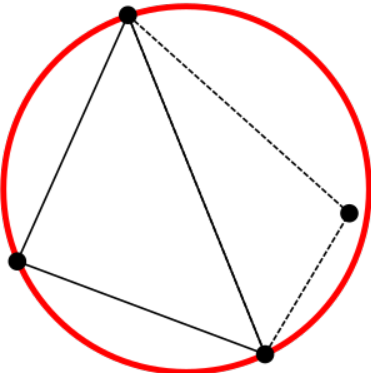
\includegraphics[width=0.44\linewidth]{no_td.png}  % Inserta la primera imagen
			\caption{Primera imagen}
			
		\end{minipage}\hfill
		\begin{minipage}{0.45\textwidth}
			\centering
			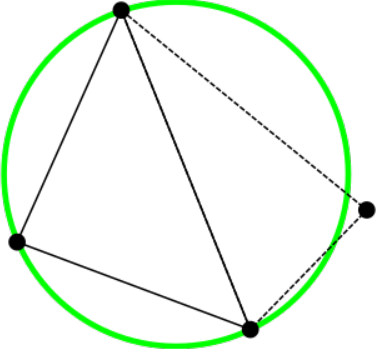
\includegraphics[width=0.5\linewidth]{si_td.png}  % Inserta la segunda imagen
			\caption{Segunda imagen}
		\end{minipage}
	\end{figure}

	
	Un resultado importante es analizar si una triangulación de Delaunay es correcta o no, para esto se utiliza la fórmula de Euler ya que dado un conjunto P de n puntos , si una cantidad h de ellos se encuentran en la envoltura convexa se optiene por dicha fórmula que  la triangulación de Delaunay tiene 2n-2-h triángulos y 3n-3-h aristas(30 sensor)
	
\section{Test de detección de patrones DIAG y LINE en el sistema PassPoint basado en los ángulos máximos de los triángulos de Delaunay  }
	
\chapter{Metodología}
Describe la metodología utilizada en tu investigación, incluyendo los métodos, herramientas y procedimientos.

\chapter{Resultados}
Presenta los resultados obtenidos durante tu investigación.

\chapter{Discusión}
Analiza los resultados y compara con otros estudios o referencias relevantes.

\chapter{Conclusiones y Recomendaciones}
Resume los hallazgos principales y ofrece recomendaciones futuras.

% Bibliografía
\addcontentsline{toc}{chapter}{Bibliografía}
\bibliographystyle{plain}
\begin{thebibliography}{9}
	\normalsize{
	\bibitem{1} Wiedenbeck, S.; Waters, J.; Birget, J.C.; Brodskly, A.; Memon, N.:\textit{ Passpoints: Design and
	longitudinal evaluation of a graphical pass- word system}. International Journal of Human-Computer
	Studies, Vol. 63(1-2):102-127, 2005.

	\bibitem{2} Sunil, S.S; Prakash, D.; Shivaji, Y.R.:\textit{ Cued click points: Graphical password authentication technique
	for security.} International Journal of Computer Science and Information Technologies, 5(2), 2014.

	\bibitem{3} Rodríguez, O.:\textit{Algoritmo para la detección de claves débiles en la técnica de autenticación gráfica passpoints}. Tesis presentada en opción al título Máster en Ciencias Matemáticas, Universidad de la
	Habana, Facultad de Matemática y Computación, Instituto de Criptografía, 2019.

	\bibitem{4} Rodríguez, O.; Legón, C.M.; Socorro, R.: \textit{Seguridad y usabilidad de los esquemas y técnicas de autenticación gráfica.} Revista Cubana de Ciencias Informáticas, Vol. 12, No. Especial UCIENCIA,
	13-27, 2018.
	
	\bibitem{5} Sonia Chiasson; Alain Forge; Robert Biddle:\textit{User interface design affects security:Patterns in
	click-based graphical passwords}.School of Computer Science and Human Oriented Technology
	Lab.Carleton University
	
	\bibitem{6}Herrera, J.A.; Suárez, L.; Legón, C.M.; Piñeiro, L.R.; Rojas, O.; Sosa, G.\textit{ Effectiveness of Some Tests of Spatial Randomness in the Detection ofWeak Graphical Passwords in Passpoint}. In \textit{Computer Science and Health Engineering in Health Services}; Marmolejo-Saucedo, J.A., Vasant, P., Litvinech, I., Rodriguez-Aguilar, R., Martinez-Rios, F., Eds.; COMPSE 2020; Lecture Notes of the Institute for Computer Sciences, Social Informatics and Telecommunications Engineering; Springer: Cham, Switzerland, 2020; Volume 359.
	
	\bibitem{7}Herrera, J.A.; Legón, C.M.; Suárez, L.; Piñeiro, L.R.; Rojas, O.; Sosa, G. Test for Detection of Weak Graphic Passwords in Passpoint Based on the Mean Distance between Points.\textit{ Symmetry} 2021,13, 777
	
	\bibitem{8}Suárez, L; Legón, C.M.; Herrera, J.A; Socorro, R.; Rojas, O.; Sosa,
	G.: \textit{Weak PassPoint passwords detected by the perimeter of Delaunay triangles}. Enviado a publicación 16 Marzo 2021, Journal Sensors. Se	encuentra en fase de revisin, pendiente de aceptación.
	
	\bibitem{9}L. Suárez. \textit{Test para la detección de contraseñas gráficas débiles en PassPoint, basado en el promedio de los	perímetros de los triángulos de Delaunay}. Master’s thesis, Universidad de la Habana, 2021.
	
	\bibitem{10} Aplicacion conjunta
	
	\bibitem{11} Herrera, J.A.; Suárez, L.; Legón, C.M.; Sosa, G. and O. Rojas: \textit{New test to detect clustered graphical passwords   in Passpoints, based on the perimeter of the convex hull}. Information 2024, 15, 447
	
	\bibitem{12} Chiu, S.N.\textit{ Spatial point pattern analysis by using Voronoi diagrams and Delaunay tessellations-A comparative study.} Biometr. J.
	2003, 45, 367–376.
	
	\bibitem{13} L. Suárez, J. A. Herrera, C. M. Legón, G. Sosa, and O. Rojas. \textit{Detection of DIAG and LINE Patterns in PassPoints Graphical Passwords Based on the Maximum Angles of Their Delaunay Triangles}.\textit{Sensors}, 22
	(5), 2022a.
	
}
\end{thebibliography}


% Anexos (opcional)
\appendix
\chapter{Anexo A}
Incluye aquí cualquier información adicional como encuestas, gráficos, o tablas complementarias.

\end{document}